\chapter{迈克耳孙干涉仪}\label{ch:b2:michelson}

1887 年，迈克耳孙与莫雷将一束光分成两束，使
两束光分别沿相互垂直的两臂传播，再使其重新会合，并观察
条纹的移动——地球穿过以太运动所应产生的移动——
结果什么也没有动，物理学随之改变。2015 年，同一台
仪器——两臂如今长四千米，经折叠后等效为一千米——
记录到一道引力波，使两臂长度
改变了质子直径的千分之一。两个年份之间，
\omterm{def:b2:michelson:instrument}{迈克耳孙干涉仪}以波长为尺度测定米的长度，分辨出
谱线，并成为精密光学的标准工具。
本章将介绍其两种构型——空气劈尖
与平行平板——并说明其条纹如何测量长度、
折射率与光谱。

\section{仪器}

\begin{definition}[迈克耳孙干涉仪]\label{def:b2:michelson:instrument}
\index{迈克耳孙干涉仪}\index{分束器}\index{补偿板}
一块\emph{分束器} $Sp$——带半反射面的玻璃板
——以 \qty{45}{\degree} 角放置，将入射光束分为两束：一束射向
反射镜 $M_1$，另一束射向 $M_2$，两镜均与各自光束垂直；
光束反射后各自返回 $Sp$，其中一半被送向
观察者，两束光在此干涉。一块\emph{补偿板}
$C$ 与分束器完全相同且与之平行，置于
原本只穿过一次分束器玻璃的那一臂中，使两束光
穿过的玻璃厚度相同，于是\omterm{thm:b2:two-wave-interference:formula}{光程差}纯粹是空气光程之差，
对所有波长都相同——这正是白光条纹所要求的。
两反射镜到 $Sp$ 的距离分别为 $d_1$
和 $d_2$；其中一面反射镜装在测微螺杆上，并配有
倾斜调节螺钉。
\end{definition}

\begin{proposition}[等效装置]\label{prop:b2:michelson:equivalent}
\index{空气劈尖（迈克耳孙）}\index{空气平板（迈克耳孙）}
从观察者一侧看，该干涉仪等效于反射镜
$M_2$ 与 $M_1'$（即 $M_1$ 在分束器中的像）：一层薄空气
夹在两反射面之间，厚度 $e = |d_1 - d_2|$，其两束反射光
发生干涉（\omterm{prop:b2:two-wave-interference:film}{分振幅}）：
\begin{itemize}
  \item $M_1' \parallel M_2$：厚度为 $e$ 的\emph{空气平板}——\omterm{prop:b2:michelson:rings}{等倾环}，
        定域于无穷远，$\delta = 2e\cos i$；
  \item $M_1'$ 以小角 $\alpha$ 相对 $M_2$ 倾斜：\emph{空气劈尖}
——等厚直条纹，定域于
        反射镜附近（劈尖处），垂直入射时 $\delta = 2\alpha x$，
        条纹间距为 $\lambda/2\alpha$。
\end{itemize}
在\emph{接触}处（$e = 0$，$\alpha = 0$），视场均匀；对白光而言，
这是各色条纹重合的唯一位置，即“白色条纹”。
\end{proposition}

\begin{proof}
将 $M_1$ 臂折叠到 $M_2$ 臂上（反射面为 $Sp$），
两束光于是映射到同一条直线上，相当于两反射镜相距 $e$；
返回的两列波即由空气层两表面反射所得（无额外
$\lambda/2$ 的相位跃变；两者均在金属面上反射，分束器对二者的处理
完全对称，仅差一个使整幅图样平移的常数相位）。
于是可直接套用 \cref{ch:b2:two-wave-interference} 中的薄膜结果，
此时 $n = 1$。
\end{proof}

\begin{omfigure}
\begin{tikzpicture}[font=\small, x=1cm, y=1cm, >=Stealth]
  \begin{scope}
    % source and beams
    \fill (-3.6,0) circle (1.5pt); \node[font=\footnotesize] at (-3.6,0.35) {$S$};
    \draw[omDef, thick, ->] (-3.4,0) -- (-0.15,0);
    % splitter at 45 deg
    \draw[thick, fill=omExo!30, rotate around={45:(0,0)}] (-0.08,-1.3) rectangle (0.08,1.3);
    \node[font=\footnotesize] at (0.55,-1.0) {$Sp$};
    % compensator (parallel, in the arm toward M1... put near upward arm)
    \draw[thick, fill=omExo!15, rotate around={45:(0,0.9)}] (-0.06,-0.6) rectangle (0.06,0.6);
    \node[font=\footnotesize] at (0.55,1.3) {$C$};
    % mirrors
    \draw[thick] (-0.9,2.6) -- (0.9,2.6); \fill[pattern=north east lines] (-0.9,2.6) rectangle (0.9,2.75); \node[font=\footnotesize] at (1.3,2.6) {$M_1$};
    \draw[thick] (2.8,-0.9) -- (2.8,0.9); \fill[pattern=north east lines] (2.8,-0.9) rectangle (2.95,0.9); \node[font=\footnotesize] at (2.85,1.25) {$M_2$};
    % beams
    \draw[omDef, thick, ->] (0,0.15) -- (0,2.55); \draw[omDef, thick, ->] (0.15,0) -- (2.75,0);
    \draw[omThm, thick, ->] (-0.2,2.45) -- (-0.2,0.2); \draw[omThm, thick, ->] (2.65,-0.2) -- (0.2,-0.2);
    \draw[omProp, thick, ->] (0,-0.2) -- (0,-2.5);
    \node[omProp, font=\footnotesize] at (0,-2.8) {观察者};
    \draw[<->] (0.4,0.4) -- (0.4,2.5) node[midway, right, font=\footnotesize] {$d_1$};
    \draw[<->] (0.4,-0.45) -- (2.7,-0.45) node[midway, below, font=\footnotesize] {$d_2$};
  \end{scope}
  \begin{scope}[xshift=8.4cm]
    \draw[thick] (-1.6,0) -- (1.6,0); \fill[pattern=north east lines] (-1.6,-0.15) rectangle (1.6,0); \node[font=\footnotesize] at (2.0,0) {$M_2$};
    \draw[thick, omDef] (-1.6,0.8) -- (1.6,0.8); \node[omDef, font=\footnotesize] at (2.0,0.8) {$M_1'$};
    \draw[<->] (-1.9,0) -- (-1.9,0.8) node[midway, left, font=\footnotesize] {$e$};
    \node[font=\footnotesize] at (0,-0.6) {空气平板：无穷远处的环};
    \draw[thick] (-1.6,-2.4) -- (1.6,-2.4); \fill[pattern=north east lines] (-1.6,-2.55) rectangle (1.6,-2.4);
    \draw[thick, omDef] (-1.6,-2.35) -- (1.6,-1.75); \node[omDef, font=\footnotesize] at (2.0,-1.8) {$M_1'$};
    \node[font=\footnotesize] at (0,-3.0) {空气劈尖：反射镜上的条纹};
  \end{scope}
\end{tikzpicture}

{\small 左：\omterm{def:b2:michelson:instrument}{迈克耳孙干涉仪}——分束器、\omterm{def:b2:michelson:instrument}{补偿板}、
两面反射镜，一束光在射向观察者处重新会合。右：
$M_2$ 与 $M_1'$（即 $M_1$ 的像）之间的等效空气层，平行时
（环形条纹）或倾斜时（直条纹）。}
\end{omfigure}

\section{两类干涉条纹}

\begin{proposition}[空气平板的环]\label{prop:b2:michelson:rings}
\index{等倾环}\index{海丁格条纹}
当 $M_1' \parallel M_2$ 且光源为\omterm{prop:b2:two-wave-interference:spatial}{扩展光源}时，观察者（或
焦距为 $f$ 的透镜及位于其焦平面上的屏）看到同心
圆环；倾角为 $i$ 的圆环级次为 $p = 2e\cos i/\lambda$；亮环
出现在 $p$ 为整数处。中心的级次最高，$p_0 =
2e/\lambda$；在其附近 $\cos i \approx 1 - i^2/2$，因此从中心算起的第 $k$ 个亮环
（以第一个亮环为起点计数，其级次比中心低 $\varepsilon = p_0 - \lfloor p_0\rfloor$
），其半径为
\[
r_k = f\,i_k = f\sqrt{\frac{(k - 1 + \varepsilon)\lambda}e} :
\]
圆环随 $e$ 增大而变密（环数更多、更细），随 $e \to 0$ 而散开，
直至接触时成为均匀视场。移动一面反射镜 $\lambda/2$ 的距离，
使 $p_0$ 改变 1：每移动半个波长，
中心便有一个圆环新生（或被吞没）。
\end{proposition}

\begin{proof}
对平行平板，$\delta = 2e\cos i$（见\cref{ch:b2:two-wave-interference}，
$n = 1$，两次金属反射无附加 $\lambda/2$）；$2e(1 - i^2/2) =
(p_0 - k + 1 - \varepsilon)\lambda$，代入 $2e = p_0\lambda$ 得 $ei^2 = (k - 1 + \varepsilon)\lambda$。
\end{proof}

\begin{proposition}[空气劈尖的条纹]\label{prop:b2:michelson:wedge}
\index{等厚条纹（迈克耳孙）}\index{菲佐条纹}
当 $M_1'$ 倾斜一小角 $\alpha$、入射近似垂直时，
距接触线为 $x$ 的镜面处\omterm{thm:b2:two-wave-interference:formula}{光程差}为 $\delta = 2\alpha x$：
条纹为与接触线平行的直条纹，
间距为 $\lambda/2\alpha$，定域于镜面上（观察时聚焦于 $M_2$，
或用透镜使 $M_2$ 与屏共轭，将其投影到屏上）。
零级条纹位于接触线上，对每个波长都一样：
用白光时为白色（或黑色，视分束器的相位而定），
两侧伴有若干彩色条纹——
这正是找到接触位置的标志。
\end{proposition}

\begin{proof}
空气劈尖的\omterm{prop:b2:two-wave-interference:film}{等厚条纹}，$e(x) = \alpha x$。定域：
对\omterm{prop:b2:two-wave-interference:spatial}{扩展光源}，经劈尖上某一点的光线
在该点重新会合，入射近似垂直时 $\delta$ 相同。
\end{proof}

\begin{omfigure}
\begin{tikzpicture}[font=\small, x=1cm, y=1cm, >=Stealth]
  \begin{scope}
    \foreach \r in {0.35,0.62,0.82,0.98,1.12,1.25,1.37,1.48} \draw[omDef, thick] (0,0) circle (\r);
    \node[font=\footnotesize] at (0,-1.9) {圆环：$r_k \propto \sqrt{k}$};
  \end{scope}
  \begin{scope}[xshift=4.8cm]
    \foreach \x in {-1.4,-1.0,...,1.4} \draw[omDef, thick] (\x,-1.5) -- (\x,1.5);
    \node[font=\footnotesize] at (0,-1.9) {劈尖：间距 $\lambda/2\alpha$};
  \end{scope}
  \begin{scope}[xshift=10.0cm]
    \begin{axis}[omaxis, axis x line=bottom, axis y line=left, width=5.0cm, height=4.2cm, at={(0,-1.9cm)},
        xlabel={$e$（mm）}, ylabel={对比度}, xmin=0, xmax=1.2, ymin=0, ymax=1.1, xtick={0,0.29,0.58,0.87}, xticklabels={0,0.29,0.58,0.87}, ytick={0,1}, samples=200,
        xlabel style={at={(axis description cs:0.5,-0.14)}, anchor=north},
        ylabel style={at={(axis description cs:-0.12,0.5)}, rotate=90, anchor=south}]
      \addplot[omThm, thick, domain=0:1.2] {abs(cos(deg(pi*x/0.29)))};
    \end{axis}
  \end{scope}
\end{tikzpicture}

{\small \omterm{def:b2:michelson:instrument}{迈克耳孙干涉仪}的两组条纹，以及钠双线条纹的对比度随平板厚度的变化：
对比度消失，
每隔 \qty{0.29}{mm} 消失一次（首次在 \qty{0.145}{mm} 处），此时两谱线的条纹
恰好反相。}
\end{omfigure}

\section{用迈克耳孙干涉仪测量}

\begin{proposition}[长度、折射率与光谱]\label{prop:b2:michelson:measure}
\index{傅里叶变换光谱学}\index{沟槽光谱}
数出经过中心的 $N$ 条条纹，即镜面移动了 $\Delta e$ 的距离，
则 $\Delta e = N\lambda/2$，长度以波长计（测微螺旋
经标定至 \qty{0.1}{\micro m}；米本身也是这样测定的）。在一臂中
插入厚度为 $\ell$、折射率为 $n$ 的透明平板后，
附加光程 $2(n - 1)\ell$ 计入 $\delta$，条纹移动 $2(n - 1)\ell/\lambda$
个条纹，由此可测折射率（及其随压强或温度的变化，
在气室中测量）。取波长为 $\lambda$ 与 $\lambda + \Delta\lambda$ 的双线，
两组条纹随 $e$ 增大先错开、后重合，
对比度每隔
\[
\Delta e = \frac{\lambda^2}{2\Delta\lambda} :
\]
即近邻谱线的分裂。更一般地，对比度
随 $e$ 变化描出光源的光谱（对比度
在 $e \sim \ell_c/2$ 的尺度上衰减）：一边扫描 $e$，一边记录中心处的强度，
即\emph{\omterm{prop:b2:michelson:measure}{傅里叶变换光谱学}}，是红外光谱仪所用的方法。
%
\end{proposition}

\begin{proof}
中心处的级次为 $2e/\lambda$，每条谱线各有其级次。两组
条纹再次重合的条件是 $2e/\lambda - 2e/(\lambda + \Delta\lambda) = 1$，即 $2e\Delta\lambda
/\lambda^2 = 1$；两组条纹在中途反相。一般的结论
见\cref{exo:b2:scalar-light-model:10}中的对比度公式。
\end{proof}

\begin{example}[钠双线与米]\label{ex:b2:michelson:sodium}
钠双线（$\Delta\lambda = \qty{0.6}{nm}$，波长 \qty{589}{nm}）：圆环时而模糊、时而清晰，
每隔 $\Delta e = 589^2/(2 \times 0.6)$ nm $= \qty{0.29}{mm}$ 一次——这是测量 $\Delta\lambda$ 的经典方法，
用螺旋可测到百分之几的精度。迈克耳孙于 1892 年
用镉的红色谱线数出标准米长度内的
$1\,553\,163.5$ 个波长，这是米与原子之间的首次联系；
今天米由 $c$ 与秒来定义；
干涉仪在生产中检验量块，
精度达到纳米量级。
\end{example}

\begin{omfigure}
\begin{tikzpicture}
\begin{axis}[omaxis, axis x line=bottom, axis y line=left, width=13.6cm, height=4.4cm,
    xlabel={$e$（\unit{\micro m}）}, ylabel={中心处 $I$}, xmin=0, xmax=6, ymin=0, ymax=2.3, xtick={0,1,2,3,4,5,6}, ytick=\empty, samples=600,
    xlabel style={at={(axis description cs:0.5,-0.14)}, anchor=north},
    ylabel style={at={(axis description cs:-0.04,0.5)}, rotate=90, anchor=south}]
  \addplot[omDef, thick, domain=0:6] {1+exp(-(x/2.2)^2)*cos(deg(2*pi*x/0.55))};
  \addplot[omThm, thick, dashed, domain=0:6] {1+exp(-(x/2.2)^2)};
  \addplot[omThm, thick, dashed, domain=0:6] {1-exp(-(x/2.2)^2)};
\end{axis}
\end{tikzpicture}

{\small 圆环中心处的强度随平板厚度增大而变化，
对\omterm{prop:b2:scalar-light-model:coherence}{相干长度}有限的光源，条纹在
$e \sim \ell_c/2$ 范围内逐渐消失；包络即光谱的傅里叶变换。}
\end{omfigure}

\begin{remark}[未测到效应的臂与测到波的臂]\label{rem:b2:michelson:history}
\index{迈克耳孙–莫雷实验}\index{引力波探测器}
迈克耳孙与莫雷曾预期，地球穿越以太的速度 $v$ 会使与之平行的那一臂的
往返时间改变 $(L/c)(v/c)^2$，
相对于垂直臂而言，条纹移动量为
$2L(v/c)^2/\lambda \approx 0.4$ 条，取 $L = \qty{11}{m}$，$v = \qty{30}{km/s}$；
转动仪器本应使图样移动相同的量。
他们本可分辨 $0.01$ 条，结果却什么也没有观察到。今天的\omterm{rem:b2:michelson:history}{引力波
探测器}是臂长为 \qty{4}{km} 的\omterm{def:b2:michelson:instrument}{迈克耳孙干涉仪}，光在每臂中往返
约三百次，并以足够稳定的激光，读出臂长的
变化 $\Delta L/L \sim 10^{-21}$ ——$10^{-18}$ m，
约为一个质子的千分之一，须克服地震运动
与光子自身的噪声。
\end{remark}

\begin{method}[使用迈克耳孙干涉仪]\label{met:b2:michelson:method}
（1）判断装置类型：平行板（圆环位于无穷远；
用透镜或眼睛在无穷远处观察）或劈尖（条纹位于
镜面上；聚焦于 $M_2$）。（2）写出 $\delta = 2e\cos i$ 或 $2\alpha x$ 及
级次。（3）将每次测量换算为条纹数：$\Delta e = N\lambda/2$，
对平板为 $2(n - 1)\ell$，对双线为 $\lambda^2/2\Delta\lambda$。（4）取
接触位置（$e = 0$，白色条纹）作为绝对参考；
注意圆环半径随 $e$ 增大而\emph{缩小}。（5）相干限制：
圆环可见的条件是 $2e < \ell_c$；劈尖要求
近似垂直入射。
\end{method}

\section{练习}

\begin{exercise}[$\star$]\label{exo:b2:michelson:1}
钠光（$\lambda = \qty{589}{nm}$）下的\omterm{def:b2:michelson:instrument}{迈克耳孙干涉仪}，将反射镜移动
\qty{0.10}{mm}：求穿过中心的圆环数；求
相当于 $250$ 条条纹的位移；若能
读出十分之一条条纹，求 $e$ 的精度。
\end{exercise}

\begin{exercise}[$\star$]\label{exo:b2:michelson:2}
平行平板厚度 $e = \qty{0.50}{mm}$，透镜焦距 $f = \qty{1.0}{m}$，$\lambda =
\qty{589}{nm}$：求中心处的级次；中心是亮的吗？求
前三个亮环的半径；当 $e$ 减小
到 \qty{0.05}{mm} 时，圆环如何变化？
\end{exercise}

\begin{exercise}[$\star$]\label{exo:b2:michelson:3}
空气劈尖，$\alpha = \qty{1.0e-4}{rad}$，$\lambda = \qty{633}{nm}$：求条纹间距；
求 \qty{2}{cm} 镜面上的条纹数；若劈角
加倍，会发生什么？如何用白光找到接触位置？
\end{exercise}

\begin{exercise}[$\star$]\label{exo:b2:michelson:4}
一臂中插入厚 \qty{0.10}{mm} 的玻璃片：对
\qty{589}{nm}、$n = 1.52$，求条纹移动量；若测得移动量为 $0.2$ 条，求
$n$ 的精度。若玻璃片厚 \qty{1}{cm}，为何
不能用白光做同样的测量？
\end{exercise}

\begin{exercise}[$\star\star$]\label{exo:b2:michelson:5}
\emph{钠双线。}（a）求圆环两次相继消失之间的厚度 $e$，
对 $\Delta\lambda = \qty{0.597}{nm}$。（b）某学生在
\qty{5.00}{mm} 内数得 $17$ 次消失：求 $\Delta\lambda$ 及其精度。
（c）在 $e = \qty{0.29}{mm}$ 处，求两谱线的级次，并验证二者相差
$\tfrac12$。（d）为何对比度从不恰好为零（两谱线
强度之比为 $2 : 1$）？求最小对比度。
\end{exercise}

\begin{exercise}[$\star\star$]\label{exo:b2:michelson:6}
\emph{空气的折射率。}一臂中长 \qty{10.0}{cm} 的气室先抽成真空，然后
缓慢充入 \qty{1}{bar} 的空气；有 $94$ 条条纹通过（$\lambda = \qty{589}{nm}$）。
（a）求空气的 $n - 1$。（b）压强变化 \qty{1}{\%} 时通过的条纹数；
若 $n - 1 \propto \rho$，求温度系数。（c）为何这一点
对任何在空气中工作的干涉仪的稳定性都很重要？（d）由
十分之一条条纹求 $n - 1$ 的精度。
\end{exercise}

\begin{exercise}[$\star\star$]\label{exo:b2:michelson:7}
\emph{\omterm{prop:b2:scalar-light-model:coherence}{相干长度}。}用低压汞灯的绿线（
\qty{546}{nm}，宽度 \qty{0.01}{nm}），圆环随 $e$ 增大而变暗。（a）求\omterm{prop:b2:scalar-light-model:coherence}{相干
长度}；求对比度可忽略的厚度 $e$。（b）用
高压汞灯（$\Delta\lambda = \qty{1}{nm}$）重做上题。（c）用氦氖激光器
（$\Delta\nu = \qty{1}{MHz}$）：当 $e = \qty{10}{m}$ 时，是否仍能看到圆环？（d）是什么
限制了白光条纹只能在接触位置附近 $\pm2$ 级之内出现？
\end{exercise}

\begin{exercise}[$\star\star$]\label{exo:b2:michelson:8}
\emph{\omterm{def:b2:michelson:instrument}{补偿板}。}若无 $C$，一束光穿过分束器的
玻璃（$e_g = \qty{5}{mm}$，$n = 1.52$）三次，另一束只穿过一次。（a）
求多出的光程；对单色光，能否通过移动反射镜
来补偿？（b）对白光为何不行（色散：$n$
在可见光范围内变化 $0.01$）？（c）
$C$ 与 $Sp$ 的平行度应达到什么公差，能保持白光条纹（取
厚度的残余差 $< \qty{0.3}{\micro m}$）？（d）现代分束器
多为薄膜或立方体，那时为何不再需要 $C$？
\end{exercise}

\begin{exercise}[$\star\star$]\label{exo:b2:michelson:9}
\emph{\omterm{rem:b2:michelson:history}{迈克耳孙–莫雷实验}。}臂长 $L = \qty{11}{m}$（折叠），$\lambda = \qty{550}{nm}$，
地球的轨道速率 $v = \qty{30}{km/s}$。（a）在以太理论中，
沿与 $\vect v$ 平行的臂的往返时间为 $2L/c(1 - v^2/c^2)$，
垂直臂的往返时间为 $2L/c\sqrt{1 - v^2/c^2}$；求二者之差，取到最低
阶。（b）将仪器转过 \qty{90}{\degree}时的预期条纹移动量
（两臂角色互换）。（c）若能探测 $0.01$ 条条纹，求
$v$ 的上界。（d）零结果说明了什么？爱因斯坦
得出了什么结论？
\end{exercise}

\begin{exercise}[$\star\star\star$]\label{exo:b2:michelson:10}
\emph{傅里叶光谱术。}圆环中心的光强
为 $I(e) = \int S(\nu)[1 + \cos(4\pi\nu e/c)]\dd\nu$，光源光谱为
$S(\nu)$。（a）对单一谱线，求 $I(e)$；求其在 $e$ 中的周期。（b）对高斯
谱线，宽度为 $\Delta\nu$：证明条纹具有
宽度 $\sim c/2\Delta\nu$、沿 $e$ 方向的高斯包络（承认高斯
函数的傅里叶变换仍是高斯函数）。（c）分辨：相距 $\Delta\nu$ 的两谱线可被分开，若
扫描达到 $e_{\max} \approx c/2\Delta\nu$；对 $e_{\max} = \qty{10}{cm}$，
求分辨本领 $\lambda/\Delta\lambda$（在 \qty{1}{\micro m} 处）。（d）为何此方法
在红外波段更受青睐（信号、“复用”优势）？
\end{exercise}

\begin{exercise}[$\star\star\star$]\label{exo:b2:michelson:11}
\emph{\omterm{rem:b2:michelson:history}{引力波探测器}。}臂长 $L = \qty{4}{km}$，光经循环利用
往返 $N = 300$ 次，$\lambda = \qty{1064}{nm}$，引力波使两臂
以相反方向改变 $\Delta L/L = 10^{-21}$。（a）求\omterm{thm:b2:two-wave-interference:formula}{光程差}的变化
及相移。（b）仪器维持在暗条纹上，测量
微弱光强 $I = I_0\sin^2(\Delta\varphi/2)$：求信号引起的
光强变化。（c）若循环光功率为 \qty{100}{W}，波长为 \qty{1064}{nm}，求
每秒光子数；求 \qty{1}{ms} 内的光子噪声（$\sqrt N$）与信号相比
如何：能否探测到？增大功率能带来什么？（d）为何两臂
长达千米，且反射镜要悬挂起来？
\end{exercise}

\begin{exercise}[$\star\star\star$]\label{exo:b2:michelson:12}
\emph{定域。}（a）对于劈尖，证明：设 $P$ 为 $M_2$ 上一点，
自该点射向无穷远处观察者（入射角为 $i$）的两条光线，
其\omterm{thm:b2:two-wave-interference:formula}{光程差}为 $2e(P)\cos i$ 与一项 $\propto\alpha i$ 之和，该项在 $i = 0$ 时抵消，
故干涉条纹仅在垂直入射时位于镜面上。（b）
一\omterm{prop:b2:two-wave-interference:spatial}{扩展光源}照明劈尖，入射角上限为
$i_{\max}$，为使干涉条纹保持清晰，$i_{\max}$ 须满足何条件
（视场边缘处 $2e\,i_{\max}^2/2 < \lambda/4$，$e = \qty{20}{\micro m}$）？（c）
对于平行平板，眼睛移动时圆环并不移动，
这是为什么？（d）一名学生移动头部时看到条纹发生漂移：
她处于哪种装置，应调节什么？
\end{exercise}

\begin{omfigure}
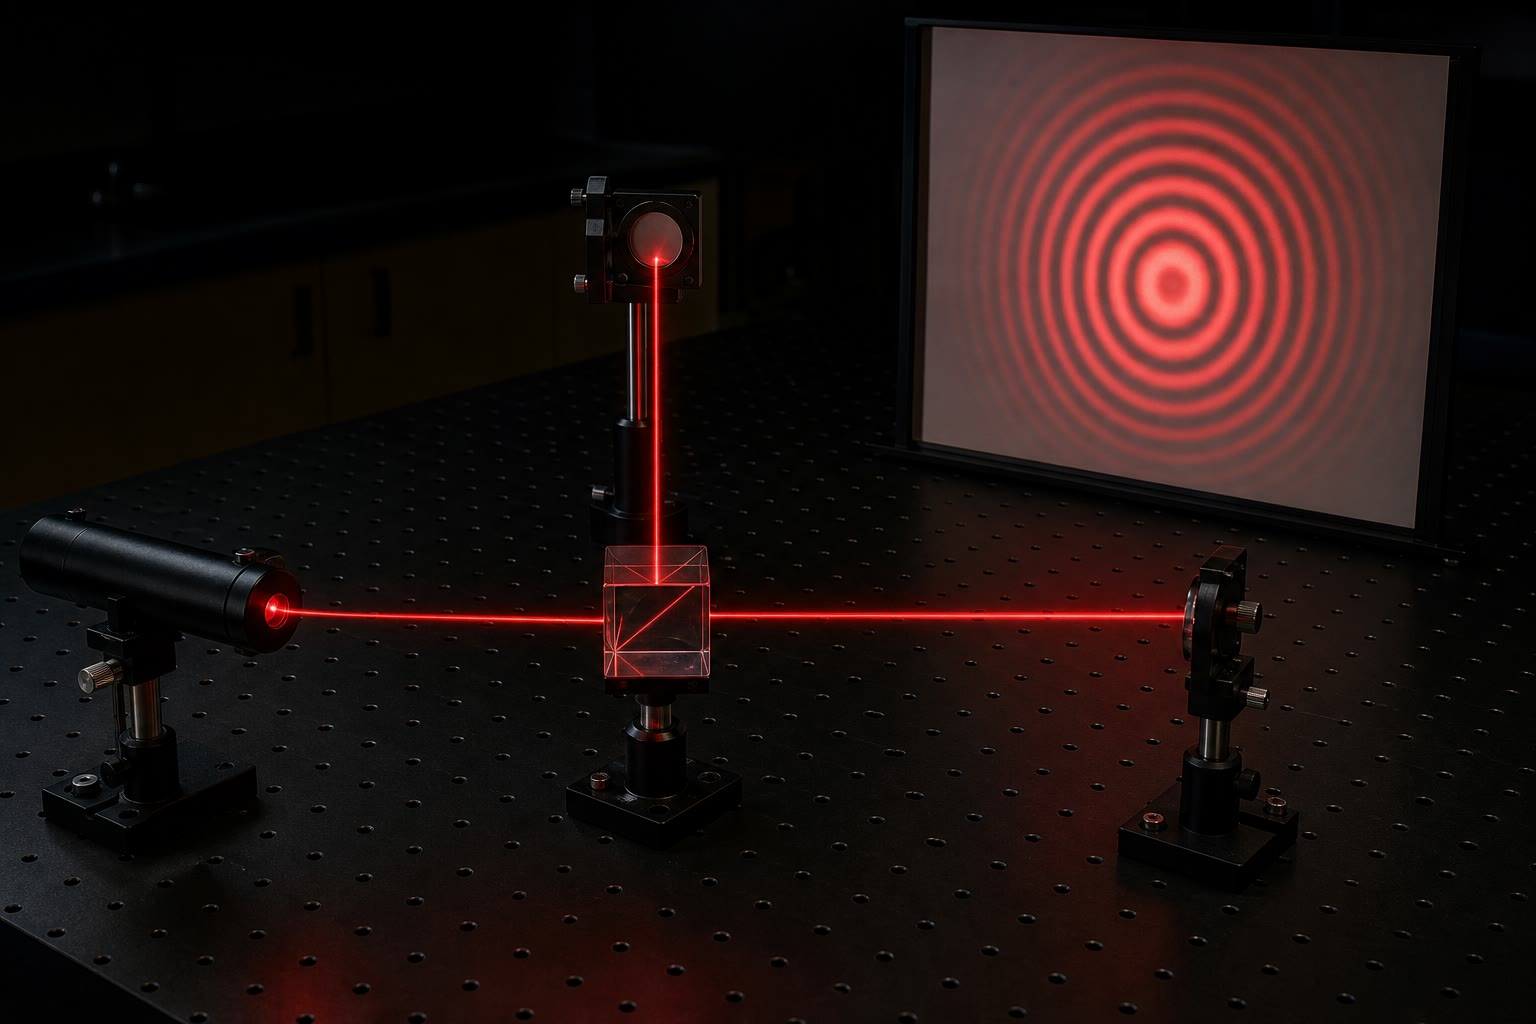
\includegraphics[width=0.58\linewidth]{images/book4/ai/b4-20-michelson-lab.jpg}

{\small 教学台上的\omterm{def:b2:michelson:instrument}{迈克耳孙干涉仪}：激光器、分束器（立方体）、两面平面镜，以及屏幕上空气平板形成的等倾圆环。}
\end{omfigure}

\begin{omfigure}
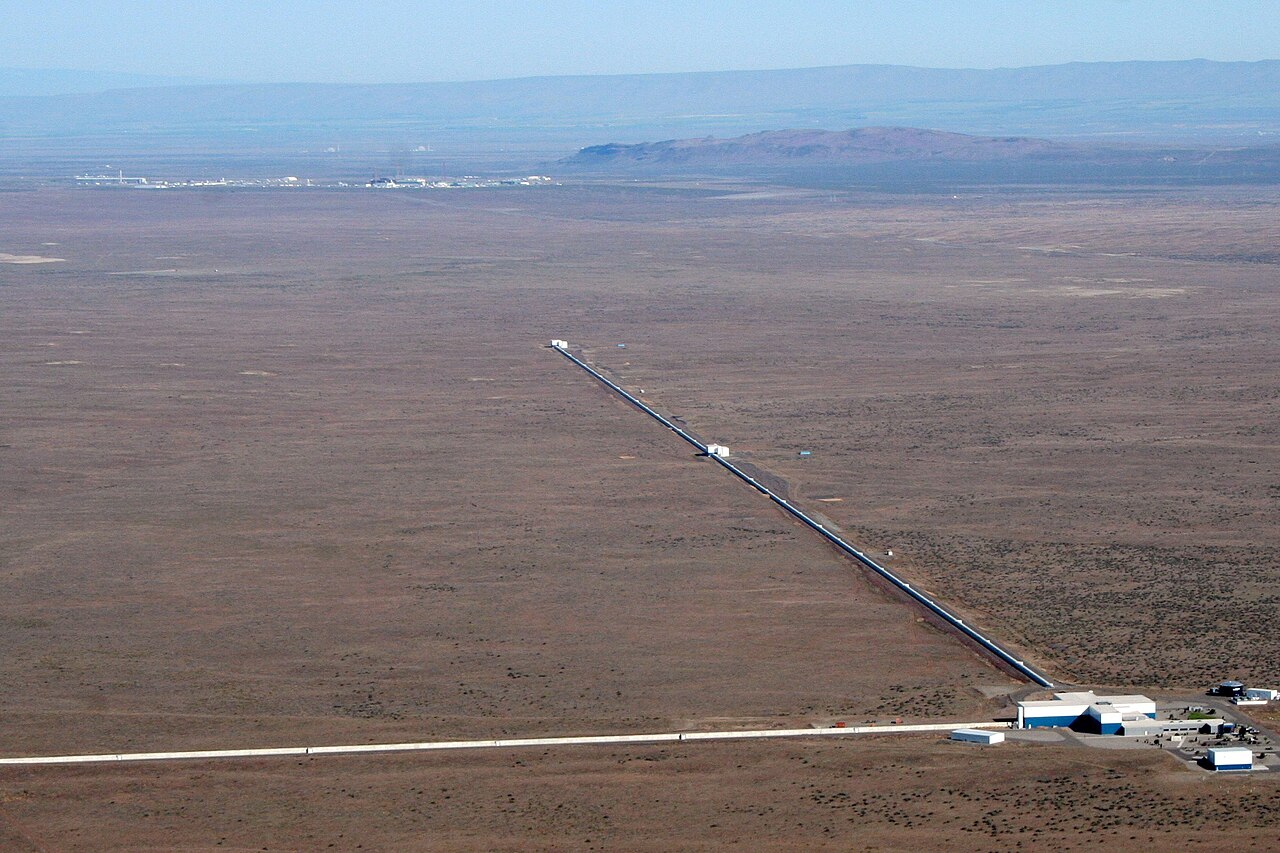
\includegraphics[width=0.6\linewidth]{images/book4/ligo-hanford-aerial.jpg}

{\small 汉福德的 LIGO 干涉仪：一台臂长四千米的\omterm{def:b2:michelson:instrument}{迈克耳孙干涉仪}，它在 2015 年记录到臂长变化量为质子直径的千分之一——即引力波的经过（LIGO 实验室）。}
\end{omfigure}

\section{问题：钠双线与空气的折射率}

\begin{problem}[{周末问题——迈克耳孙干涉仪上的一次完整测量：
寻找接触、读取长度、分辨
黄线双线、测定空气折射率}]
\label{pb:b2:michelson:1}

干涉仪的测微螺杆分度值为 \qty{1}{\micro m}；
钠灯给出 $\lambda_1 = \qty{589.0}{nm}$ 与 $\lambda_2 = \qty{589.6}{nm}$ 两条谱线，
强度之比为 $2 : 1$；另有白光灯与 He--Ne 激光器（\qty{632.8}{nm}）
亦可供使用。

\medskip
\noindent\textbf{第一部分——装置调节。}
\begin{enumerate}
  \item 用激光器时，学生在卡片上看到两臂的两个光斑，
        她用倾斜螺钉使两者重合，随即看到
        直条纹：这是哪种配置？其间距说明残余倾斜的
        大小（间距 \qty{2}{mm}）为何？
  \item 转动倾斜螺钉时，条纹先弯曲，随后变为
        圆环：为何会出现圆环？此时 $M_1'$ 位于何处？
  \item 她平移镜子，数得中心吞没了 $158$ 个圆环：
        求位移量；$e$ 正在朝哪个方向变化？
  \item 她继续平移，圆环扩散，中心斑扩大，
        直至充满视场：她到达了什么状态？换用钠灯代替激光器后，
        她看不到任何特殊现象：为何如此？白光下为何在此处
        出现居中的亮条纹，
        两侧为彩色条纹？
  \item 她在接触时将 $M_1$ 微微倾斜，于白光下看到
        直的彩色条纹：请说明原因，并给出中央白色条纹两侧
        各可期望看到多少条。
  \item 激光光斑直径为 \qty{10}{mm}，她希望在焦距为 $f = \qty{20}{cm}$ 的
        透镜视场中看到十个圆环（$\lambda = \qty{632.8}{nm}$）：
        所需厚度 $e$ 为多少（用第 $k$ 个圆环的半径）。
  \item 为何\omterm{def:b2:michelson:instrument}{补偿板}须与分束器平行，
        若将其移去，白光下她会看到什么？
\end{enumerate}

\medskip
\noindent\textbf{第二部分——双线。}
\begin{enumerate}[resume]
  \item 从钠灯下的接触位置出发，她增大 $e$：
        圆环的对比度下降、消失，之后又恢复。求第一次消失时的
        厚度，以及第 $n$ 次消失时的厚度。
  \item 她记录了 $12$ 次消失，其厚度范围自 $e = \qty{0.15}{mm}$ 至
        $e = \qty{3.35}{mm}$（首末读数取自螺杆）：求
        $\Delta\lambda$，并求每次读数精确到 \qty{5}{\micro m} 时的精度。
  \item 求两谱线在第一次消失处的级次 $p_1$ 与 $p_2$，
        以及在首次恢复满对比度处的级次。
  \item 给定强度比 $2 : 1$，求消失处的最小对比度
        （较弱谱线的条纹仍然存在）。
  \item 在谱线的自然宽度（各为 \qty{0.02}{nm}）将条纹全部抹去之前，
        她能数出多少次消失？
  \item 若光源具有三条等间距谱线，将呈现什么现象？
\end{enumerate}

\medskip
\noindent\textbf{第三部分——空气。}
将一长度为 $\ell = \qty{5.00}{cm}$ 的带玻璃窗气室置于一臂中，
抽空后缓慢充入空气，同时
对激光条纹计数。
\begin{enumerate}[resume]
  \item 气室充至 \qty{1}{atm} 时产生的\omterm{thm:b2:two-wave-interference:formula}{光程差}，
        若 $n - 1 = \qty{2.9e-4}{}$，求条纹数。
  \item 她数得 $46$ 条条纹：求其测得的 $n - 1$ 值。
  \item 她仅充入 \qty{0.20}{bar}：预期会看到多少条纹
        （$n - 1 \propto$ 压强）。
  \item 测量期间室温升高 \qty{3}{K}，两臂中各有
        \qty{40}{cm} 的敞开空气光路，其折射率每开尔文变化
        $-\qty{1e-6}{}$：求条纹漂移量，并判断它
        对第二部分、第三部分是否构成问题？
  \item 为何气室的玻璃窗不会使测量产生偏差
        （它们在整个计数过程中始终在位）？
  \item 以 CO$_2$ 重复实验（$n - 1 = \qty{4.5e-4}{}$）：
        求充满气室时的条纹数，
        并说明仅凭计数如何辨别该气体。
\end{enumerate}

\medskip
\noindent\textbf{第四部分——局限性。}
\begin{enumerate}[resume]
  \item 螺杆读数精确到 \qty{1}{\micro m}：比较以条纹计数
        在 \qty{1}{cm} 范围内测得的长度精度，
        与仅用螺杆测量的精度相比如何。
  \item 一面镜子受到振幅为 \qty{50}{nm}、频率为 \qty{100}{Hz}
        的振动：求条纹的运动，人眼看到什么，
        以每秒 $25$ 帧拍摄的照相机又看到什么？
  \item 激光器频率在计数期间相对漂移 \qty{1e-8}{}，
        在 $e = \qty{1}{cm}$ 的计数过程中，求条纹数的误差。
  \item 一块 \qty{10}{mm} 的量块经干涉法检定可达 $\lambda/20$，
        求其绝对精度与相对精度。
  \item 为何测量长度时常选用\omterm{def:b2:michelson:instrument}{迈克耳孙干涉仪}，
        而测量光谱时则选用衍射光栅（下一章）？
  \item 总结所测的四个量（长度、双线分裂、折射率、
        \omterm{prop:b2:scalar-light-model:coherence}{相干长度}），以及得到各量所依据的
        条纹观察。
\end{enumerate}
\end{problem}
